\documentclass[main.tex]{subfiles}
\begin{document}

General Instructions. Read carefully before starting. Solve 5 problems in all; at most 2 questions may be selected from the same section. Candidates registered in the following focus areas must answer two of their five questions from the relevant section as follows:\\

\begin{itemize}
    \item Computer Architecture and High-Performance Computing: Section 1
    \item Communications & Networks: Section 3
    \item Electrical Power & Energy: Section 8
    \item Electromagnetics, Radiation Systems \& Microwave Engineering: Section 4
    \item Electronics, Photonics & MEMS: Section 6
    \item Signal \& Image Processing, Systems \& Controls: Section 3
\end{itemize}

Please write your name and student number below:\\\\

Solve each problem in a \underline{separate} blue book. Write the section number, problem number, and your student number on the front of each blue book. Do not write your name on the blue book. Submit solutions to only five \(5\) problems. Use only one blue book per problem. For each problem, make a special effort to give the answers in a clear form. The exam will begin at 10:00 a.m. and end promptly at 3:00 p.m. Only calculators provided by the department at the examination will be allowed. Personal items including cell phones and other electrical devices must be relinquished prior to the start of the examination. This is a closed book, closed notes examination.

\begin{enumerate}

\subsection{Section 1}

\item After graduating, you are asked to become the lead computer designer at New Computers Inc. You have invented a scheme that reduces the loads and stores normally associated with procedure calls and returns. The first thing you do is run some experiments with and without this optimization. Your experiments use the same state-of-the-art optimizing compiler that will be used with either version of the computer. These experiment reveal the following information:
\begin{itemize}
    \item The clock rate of the un-optimized version is 15\% higher.
    \item 45\% of the instructions in the un-optimized version are loads and stores.
    \item The optimized version executes one-third as many loads and stores as the un-optimized version.
    \item For all other instructions the dynamic execution counts are unchanged.
    \item All instructions (including load and store) take one clock cycle.
\end{itemize}
Which is faster? The optimized version or the un-optimized one. Justify your decision quantitatively by computing an improvement factor to validate your answer.

\item The IEEE 754 Floating point number standard format for single precision floating-point numbers can be summarized as follows. The 32 bits number is divided as shown in figure \ref{fig:f1}. A number is normalized if the exponent value is between 1 and 254, and is denormalized if the exponent value is 0 and the fraction value is not 0. The value of a normalized number is $(-1)^S \times (1+Fraction) \times 2^{(Exponent-bias)}$ and the value of a denormalized number is $(-1)^S \times (0+Fraction) \times 2^{(1-bias)}$. Where the bias value is 127. Please answer the following questions:

\begin{figure}
\centering\fbox{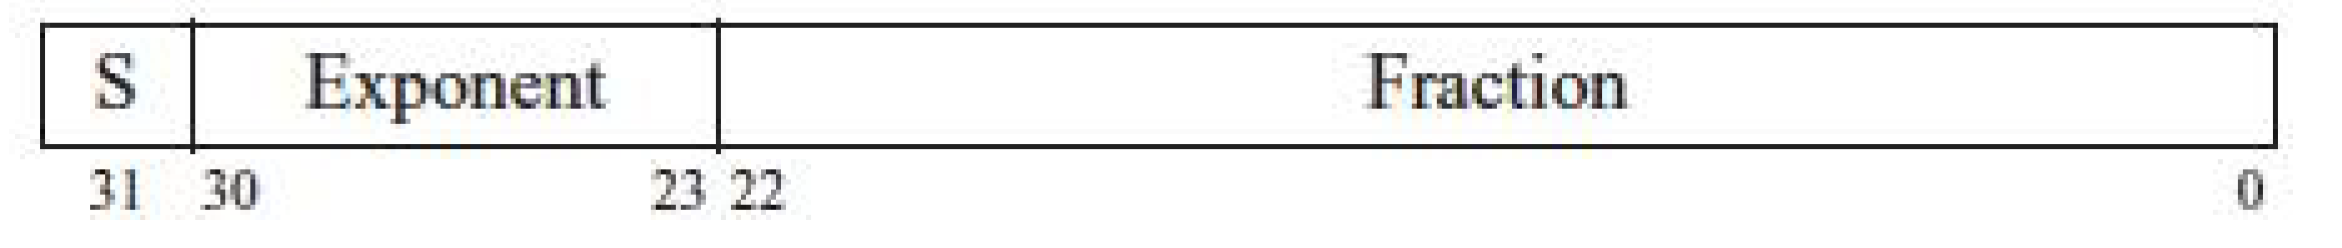
\includegraphics[width=4.0in]{figures/2018s/02q_a.png}}
\caption{32 bits number}
\label{fig:f1}
\end{figure}

\begin{enumerate}
    \item What are the maximum and minimum normalized numbers that can be computed using single precision format?
    \item What are the maximum and minimum denormalized numbers that can be computed using single precision format?
    \item If we change the Exponent size to be 10 bits instead of 8 and the fraction to be 21 bits instead of 23 bits:
    \begin{enumerate}
        \item What should the bias value be?
        \item Repeat question 2 (wording confusing assume 2a) for the new format.
        \item Repeat question 3 (wording confusing assume 2b) for the new format
    \end{enumerate}
    \item Represent the following two decimal numbers in Single Precsion format:
    \begin{enumerate}
        \item 0.1
        \item 33554431
    \end{enumerate}
    \item Take the values you computed in (d) and convert them back into decimal. Did the numbers change? Explain why.
\end{enumerate}

\item For a hypothetical CPU which has 64 bit virtual address and 41 bit physical address with two levels of cache. The L1 cache is virtually indexed and physically tagged. The L1 size is 8KB. The page size is 8KB. The L2 cache is 4MB. The block size is 64 bytes. Please illustrate the translation of virtual address to physical address, as well as the interactions to the TLB and L1/L2 Cache. Indicate how many bits are used for page number, page offset, TLB index, TLB tag, cache index, cache tag, etc.

\subsection{Section 2}

\item Given \textbf{A} =
    \begin{bmatrix} 
	1 & 2 & 3 & 4 \\
	-1 & 1 & 3 & 2\\
	2 & 2 & 2 & 4 \\
	\end{bmatrix},
	\textbf{y\textsubscript{1}} =
	\begin{bmatrix} 
	2\\
	-2\\
	4\\
	\end{bmatrix},
	\textbf{y\textsubscript{2}} = 
	\begin{bmatrix} 
	1\\
	1\\
	1\\
	\end{bmatrix}

    \begin{enumerate}
        \item Find a basis for the range space of \textbf{A}, R(\textbf{A})
        \item Find a basis for the null space \textbf{A}, N(\textbf{A})
        \item Find the rank and nullity of \textbf{A}
        \item For the equation \textbf{y\textsubscript{1}} = \textbf{A}\textbf{x\textsubscript{1}}, where \textbf{x\textsubscript{1}} is a $4\times1$ vector, does a solution exist for \textbf{x\textsubscript{1}}?
        \item For the equation \textbf{y\textsubscript{2}} = \textbf{A}\textbf{x\textsubscript{2}}, where \textbf{x\textsubscript{2}} is a $4\times1$ vector, does a solution exist for \textbf{x\textsubscript{2}}?
        \item If a solution \textbf{x\textsubscript{1}} and/or \textbf{x\textsubscript{2}} exist in parts (d) and (e), find \underline{all} solutions.
    \end{enumerate}

\item For the system \textbf{A} =
    \begin{bmatrix} 
	-1 & 8\\
	0.5 & -1\\
	\end{bmatrix},
	\textbf{b} =
	\begin{bmatrix} 
	1\\
	0.5\\
	\end{bmatrix},
	\textbf{c} = 
	\begin{bmatrix} 
	-1\\
	1\\
	\end{bmatrix}
	
	\begin{enumerate}
	    \item Design a state observer;
	    \item Using the state estimates from part a), find an appropriate state feedback such that the system will have a purely oscillatory response with a natural frequency of oscillation $\omega_n = 2$ radians/second.
	\end{enumerate}
	
\item Consider a system with a transfer function 
$$\mathrm{G}(s)=\frac{(s-2)(s-5)}{(s+1)(s-3)(s+4)}$$
Is it possible, using \underline{state feedback} to change it to

    \begin{enumerate}
        \item $\mathrm{G}(s)=\frac{(s-5)}{(s+1)(s+4)}$?
        \item $\mathrm{G}(s)=\frac{s-5}{(s+1)(s+3)(s+4)}$?
    \end{enumerate}
    
If yes, do it. Are the resulting systems controllable? observable? If no, explain why not.

\subsection{Section 3}

\item A binary source generates a sequence of symbols with probabilities p and 1-p, respectively. Given the first symbol in the sequence, the source continues to generate symbols until the opposite symbol is generated. Let X denote the length of the sequence, including the first symbol.

    \begin{enumerate}
        \item Find the probability mass function of X.
        \item Find the expected value of X.
    \end{enumerate}
    
\item Messages arriving at a central office switch are exponentially distributed in length, with average length 800 bits and average arrival rate of 16 messages per second. The switch has an infinite buffer and is served by a 64 kilobit per second transmission circuit.

    \begin{enumerate}
        \item Determine the traffic intensity for the switch in Erlangs.
        \item Determine the probability distribution of the number of messages in the buffer.
        \item Determine the average waiting time of a message in the buffer in seconds.
        \item Determine the total average time a message spends in the system, including the waiting time and the service time.
    \end{enumerate}

\item Let $\{\mathrm{Xn}: \mathrm{n}=1,2 \ldots\}$ be an infinite sequence of independent binary random variables with sample values \{0,1) and P\{X n=0\} = 2/3. Let $\text{Yn}=\sum_{\text{i=1}}^{\text{n}} \text{Xi}$ be a random process defined by Xn.

    \begin{enumerate}
        \item For n=5, determine all sample functions of the random process.
        \item Determine the probability mass function of Yn.
        \item Find the expected value and variance of Yn.
        \item Find the autocorrelation function of Yn, $\mathrm{R}\{\mathrm{Y}(\mathrm{n}, \mathrm{n}+\mathrm{k})\}=\mathrm{E}\{\mathrm{Yn} \mathrm{Yn}+\mathrm{k}\}$
    \end{enumerate}
    
\subsection{Section 4}

\item The magnetic field of a particular mode in a parallel-plate air waveguide with a plate separation of 2.5 cm is given by
$$H_{z}(x, y)=C e^{-j 640 \pi x / 3} \cos (160 \pi y)$$
where x and y are both in meters.
    
    \begin{enumerate}
        \item Is this a TE\textsubscript{n} or TM\textsubscript{n} mode? What is n? Is it a propagating or non-propagating mode?
        \item What is the operating frequency?
        \item Find the corresponding electric field.
    \end{enumerate}
    
\item An electromagnetic field in free space, $\mu_{0}=4 \pi \times 10^{-7}$ henry/meter, $\varepsilon_0 = 8.85 \times 10^{-12}$ farads/meter, is specified as by the vector phasor 

$$\underline{E}(\underline{r})=\underline{E}_{0} \varepsilon^{-j \underline{k} \underline{g} \underline{r}}$$

where $\underline{E}_{0}=\hat{x}$ the unit vector in the x direction of a rectangular coordinate system (x,y,z).

$$\begin{aligned}
&\underline{r}=x \hat{x}+y \hat{y}+z \hat{z} \\
&\underline{k}=-j \hat{y}+2 \hat{z}
\end{aligned}$$

    \begin{enumerate}
        \item What is the frequency f of the electromagnetic field (Hz)?
        \item Describe the equi-phase surfaces of the field. Write a general equation for the equi-phase surfaces.
        \item Describe the constant magnitude-of-field surfaces. Write a general equation for these equal-magnitude surfaces.
        \item Evaluate the average power as a function of position.
    \end{enumerate}

\item A plane wave is incident in the interface between two dielectrics $\varepsilon_1$ and $\varepsilon_2$, $\varepsilon_1 > \varepsilon_2$ as shown in figure \ref{fig:12q_a}.

\begin{figure}
\centering\fbox{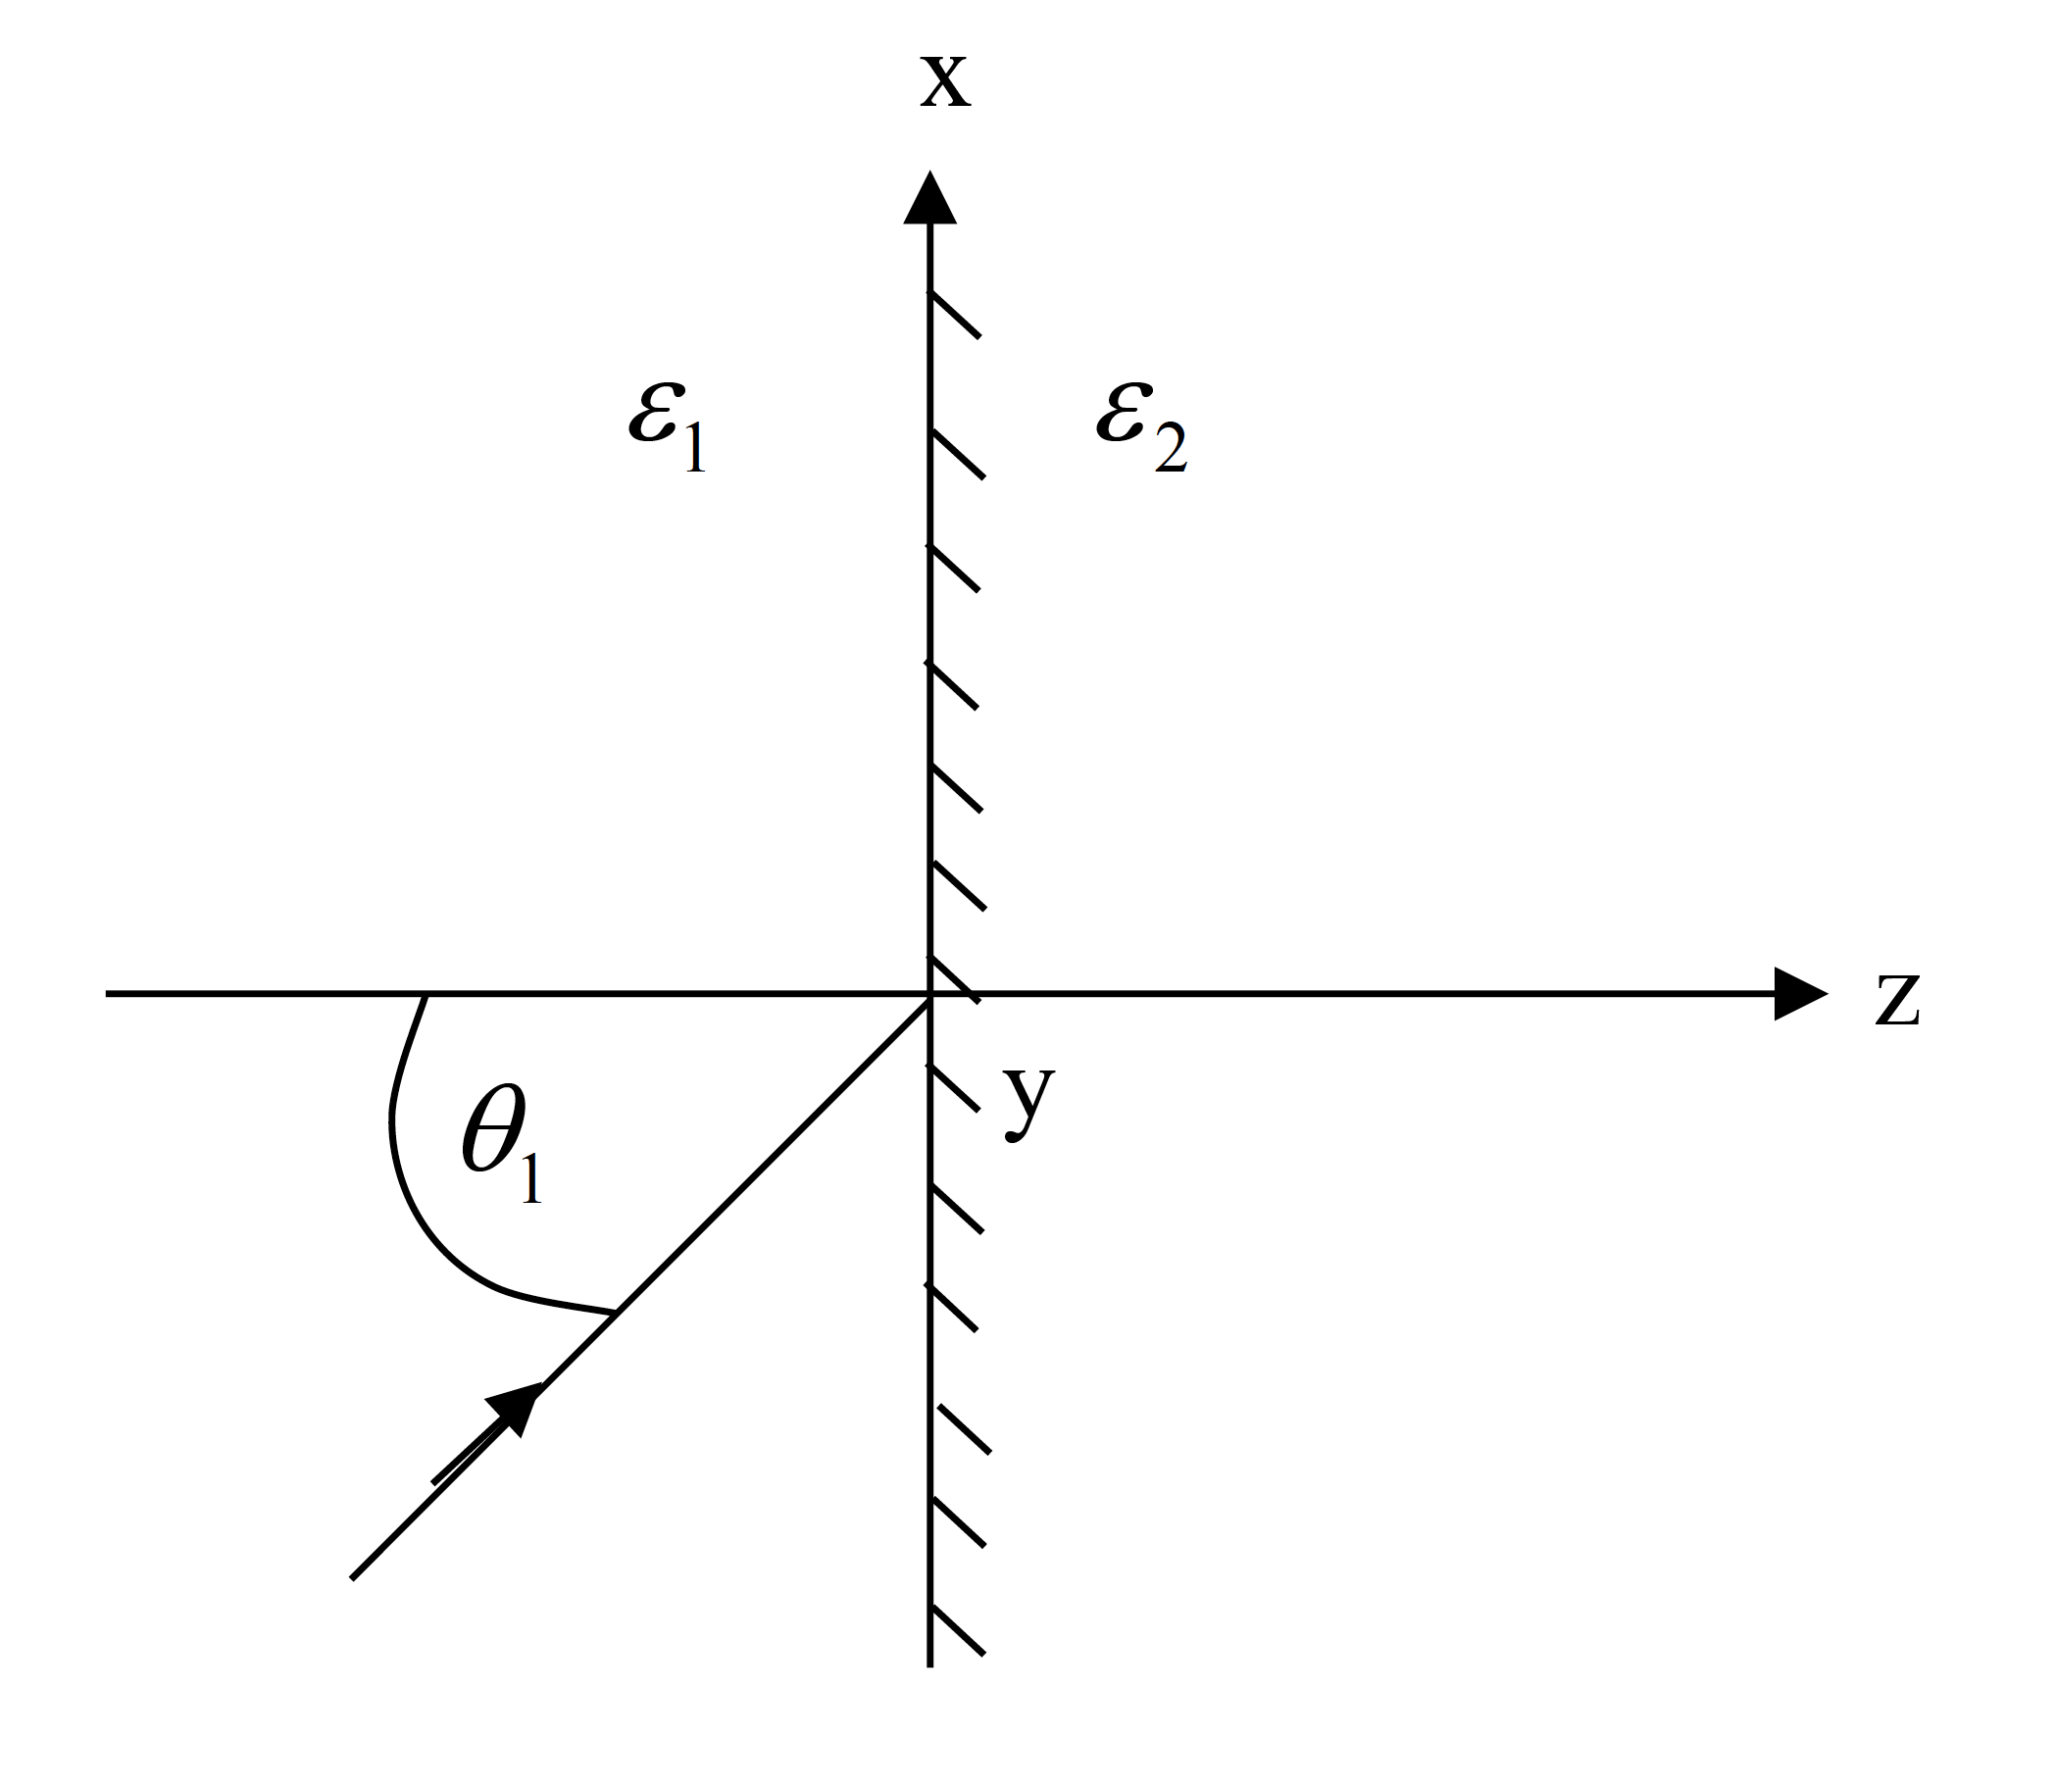
\includegraphics[width=2.0in]{figures/2018s/12q_a.png}}
\caption{Plane wave incident incident in the interface between two dielectrics}
\label{fig:12q_a}
\end{figure}

    \begin{enumerate}
        \item Find the angle $\theta_{1c}$ such that all waves incident with $\theta_1 > \theta_{1c}$ are "totally reflected".
        \item For $\theta_1 > \theta_{1c}$, describe the field (if any) in the region $z > 0$ in the $\varepsilon_2$ dielectric.
        \item If \underline{$E$} is perpendicular to the plane of the incidence, $\underline{E} = E_y \hat{y}$, find the phase of the reflection coefficient.
    \end{enumerate}

\subsection{Section 5} 

\item In the following:

    \begin{enumerate}
        \item Find the Fourier transform of 
        $$x(t)=\frac{\sin (\pi 2 B t)}{\pi 2 B t} \cos \left(2 \pi f_{c} t\right)$$
        where $f_{c}>2 B>0$.
        \item Find the Hilbert transform $\hat{x}(t) \text { of } x(t)$.
        \item Find the analytic signal $\psi(t) \text { of } x(t)$.
        \item Find the complex envelope $\gamma(t) \text { of } x(t)$.
    \end{enumerate}
    
\item Assume that $x[n]$ is a real-valued discrete-time signal and $h[n]$ is a real-valud impulse response of linear time-invariant discrete-time system. Let $y_{1}[n]=x[n] \star h[n]$ represent filtering the signal in the forward direction, where $\star$ stands for convolution. Now filter $y_{1}[n]$ backward to obtain $y_{2}[n]=y_{1}[-n] \star h[n]$. The output is then given by reversing $y_{2}[n]$ to obtain $y[n]=y_{2}[-n]$.

    \begin{enumerate}
        \item Show that this set of operation is equivalently represented by a filter with impulse response $h_{o}[n]$ as $y[n]=x[n] \star h_{o}[n]$ and express $h_{o}[n]$ in terms of $h[n]$.
        \item Show that $h_{o}[n]$ is an even signal and find the phase response of a system having impulse response $h_{o}[n]$. Is the system causal?
        \item Let $H(z)$ and $H_{o}(z)$ be z-transforms of $h[n]$ and $h_{o}[n]$, respectively, and that $h[n]$ is causal. If $H(z)=1 /\left(1-0.9 z^{-1}\right)$ find $H_{o}(z)$, the region of convergence of $H_{o}(z)$, and $h_{o}[n]$.
        \item Repeat (c) if $H(z)=1-0.9 z^{-1}$.
    \end{enumerate}
    
\item Solve the differential equation
    $$y^{\prime \prime}(t)+2 y^{\prime}(t)+y(t)=u(t-1)$$
for $t \geq 0$ using the Laplace transform. $u(t)$ is the unit step function and the initial conditions are $y\left(0^{-}\right)=y^{\prime}\left(0^{-}\right)=1$.

\subsection{Section 6}

\item Provide clear explanations to the following questions:

    \begin{enumerate}
        \item Using band-theory and energy-related arguments, explain why a metal conducts, an insulator blocks current, and a semiconductor conducts current only under certain situations.
        \item A PN junction is used as a photodetector. Assume that light is shining on all parts of the diode equally. Which part of the photodiode is most critical for photo detection and why? In this application, should the devices be under forward or reverse bias?
        \item After repeated operations of a PMOS MOSFET, hole-type interface traps are formed in the Si-SiO2 interface, does this process increase or decrease the threshold voltage? Draw the band-diagram and the sub-threshold IV curve to illustrate your answer.
    \end{enumerate}

\item MOS Capacitor

    \begin{enumerate}
        \item Draw the band diagram of a MOS system where the "metal" work function $\Phi_{\mathrm{M}}$ is larger than the silicon work function $\Phi_{\mathrm{S}}$. Assume that there are no applied voltages at the p-type substrate (doping $\mathrm{N}_{\mathrm{A}}$) and the gate. On the diagram clearly label the following parameters and functions: electron affinity in the semiconductor $\chi_{\mathrm{Sc}}$, the Fermi level $\mathrm{E}_{\mathrm{F}}$, the conduction and valance band edges $\mathrm{E}_{\mathrm{c}}$ and $\mathrm{E}_{\mathrm{V}}$, the band-gap $\mathrm{E}_{\mathrm{g}}$, the mid-gap $\mathrm{E}_{i}$, the thickness of the oxide $\mathrm{t}_{\mathrm{ox}}$, the potential drop in the oxide $\phi_{\mathrm{ox}}$, and the potential drop in the semiconductor $\phi(\mathrm{x})$
        \item For this device, what is the most likely outcome when no voltages are applied: inversion or accumulation? Why?
        \item Poly-Silicon Gate Depletion (refer to Figure \ref{fig:17q_a}): Assume the voltage $\mathrm{V}_{\mathrm{ox}} = \qty{1}{\volt}$ across a $\qty{2}{\nano\meter}$ thin \ch{SiO2} oxide. The $\mathrm{P}^{+}$ poly gate doping is $\mathrm{N}_{\text {poly }}=1 \times 10^{19} \mathrm{~cm}^{-3}$ and the substrate is n-doped with $\mathrm{N}_{\mathrm{D}}=10^{17} \mathrm{~cm}^{-3}$. Find the poly depletion width, $\mathrm{W}_{\mathrm{dep }}$.
    \end{enumerate}
    
\begin{figure}
\centering\fbox{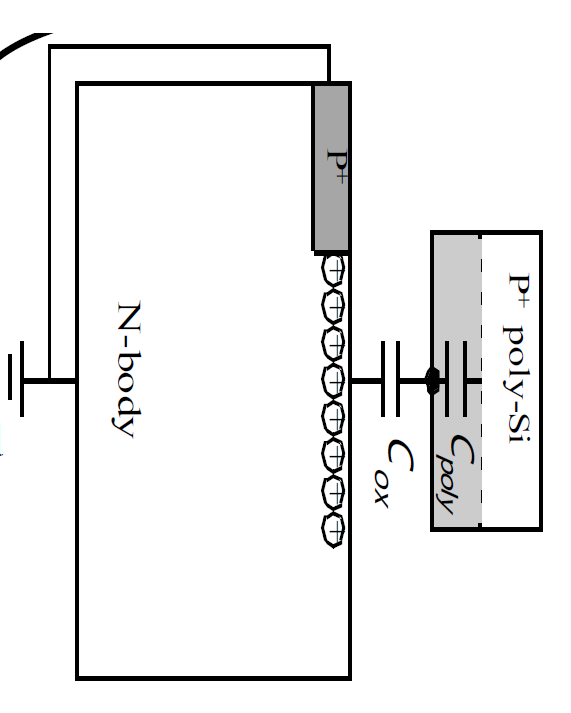
\includegraphics[width=3.0in]{figures/2018s/17q_a.png}}
\caption{Schematic of the poly depletion capacitances upon gating this MOS capacitor. $\mathrm{T}=300\mathrm{K}$}. Gate and body are Silicon. The gate ocide is \ch{SiO2}, $\mathrm{t}_{\mathrm{ox}} = 2 \mathrm{~nm}$}
\label{fig:17q_a}
\end{figure}

\item Basic \textit{pn}-junction operation.\\

Consider the ideal so-called "long-base" abrupt \textit{pn}-junction silicon diode that has a uniform cross section and constant doping on both sides of the \textit{pn}-junction. The diode is doped as follows: $\mathrm{N}_{\mathrm{a}}=8.0 \times 10^{16} \mathrm{~cm}^{-3}$ \textit{p}-type and $\mathrm{N}_{\mathrm{d}}=1 \mathrm{x} 10^{16} \mathrm{~cm}^{-3}$ \textit{n}-type. For this material, the minority-carrier lifetimes are: $\tau_{\mathrm{n}}=4 \times 10^{-6} \mathrm{~s}$ and $\tau_{\mathrm{p}}=1 \times 10^{-6} \mathrm{~s}$, respectively. You may assume that the effects within the space-charge region are negligible and that the minority carriers flow only by diffusion in the charge neutral regions.

    \begin{enumerate}
        \item Draw/sketch the band-diagram for this system. Also, plot the electrostatic potential, the net charge density and the and the corresponding electric field.
        \item Determine the value of the built-in potential across the \textit{pn}-junction.
        \item Calculate the density of the minority carriers at the edge of the space-charge region for a forward bias of 0.3V.
        \item Under bias condition, calculate and plot the minority and majority carrier currents as a function of distance from the junction.
    \end{enumerate}

\subsection{Section 7}
	
\item Answer the following questions about LANs (wired and wireless):

    \begin{enumerate}
        \item Describe (through some pseudo code and sufficient explanation) CSMA/CD and Binary Exponential Backoff as used in IEEE 802.3 Ethernet.
        \item Describe CSMA/CA (through some pseudo code and sufficient explanation) as used in IEEE 802.11 WiFi.
    \end{enumerate}
    
\item M terminals are attached by a dedicated pair of lines to a hub in a star topology (Figure \ref{fig:20q_a}). The distance from each terminal to the hub is d meters, the speed of the transmission lines is R bits/second, all frames are f length 12,500 Bytes, and the signal propagates on the line at speed of $2.5^{*} 10^{8}$ meters/second. For M=6 terminals, d=25 meters and R = 10Gbps, what is the maximum network throughput achievable when the hub is implementing slotted ALOHA?

\begin{figure}
\centering\fbox{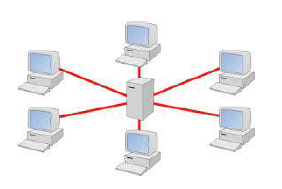
\includegraphics[width=3.0in]{figures/2018s/20q_a.png}}
\caption{Star Topology}
\label{fig:20q_a}
\end{figure}

\item Consider a data link layer with the following parameters: Frame transmission time at the sender is $\mathrm{t}_\mathrm{f}=20$ microseconds. ACK or NAK transmission time at the receiver is $\mathrm{t}_\mathrm{ack} = 10$ microseconds. Link propagation delay on both directions is $\mathrm{t}_{\mathrm{prop}} = 25$ microseconds. Suppose frame processing time at both sender and receiver is negligible, i.e., $\mathrm{t}_{\mathrm{prop}] = 0$. Finally, overall round-trip probability of frame error on the link is $r=0.04$. 

    \begin{enumerate}
        \item Assume that for the Stop-and-wait ARQ scheme, the TIMEOUT at the sender is chosen optimally. What is the resulting throughput (frames/second)?
        \item  In the Go-Back-N ARQ scheme, if the link is error free, what is the minimum window size $N$ that is able to keep the link busy?
        \item Choose window size in Part b and now consider the link error probability $r=0.04$. What the throughput (frames/second) of the Go-Back-N ARQ scheme?
    \end{enumerate}

\subsection{Section 8}

\item A three-phase 250MVA, 20kV, 60Hz salient pole synchronous machine has parameters Xd = 1.1 pu, Xq = 0.6 pu and Ra~0. The machine delivers 230MW at 0.9 lagging power factor to an infinite busbar. Calculate the excitation voltage and power angle. Draw the phasor diagram. (Hint: use per unit values and give your answers in pu).

\item A wind turbine is to be designed with an electrical power output of 7.0MW. The rated upwind free wind speed is 13 m/s. Determine the length of the rotor blades and the height of the supporting tower in meters and the rotational speed of the rotor in rev/min if the tip-speed ratio whose value as 7.0 determines the maximum Power Coefficient of 0.45. Use the density of air as $\num{1.225}\unit{kg/m^3}$

\item A 450MVA, 20kV, 60-Hz round-rotor synchronous generator has an Inertia constant H = 5s. Displayed on the axes in Figure \ref{fig:24q_a} are Torque/Angle characteristics for various faults occurring on a double circuit transmission line when connected between a synchronous generator and an infinite busbar. Using the Equal Area Criterion, determine the critical switching times for both a $3 \varphi$ fault and a Line to Line fault when the input and torque from the turbine is 1.0 pu as shown in the diagram.

\begin{figure}
\centering\fbox{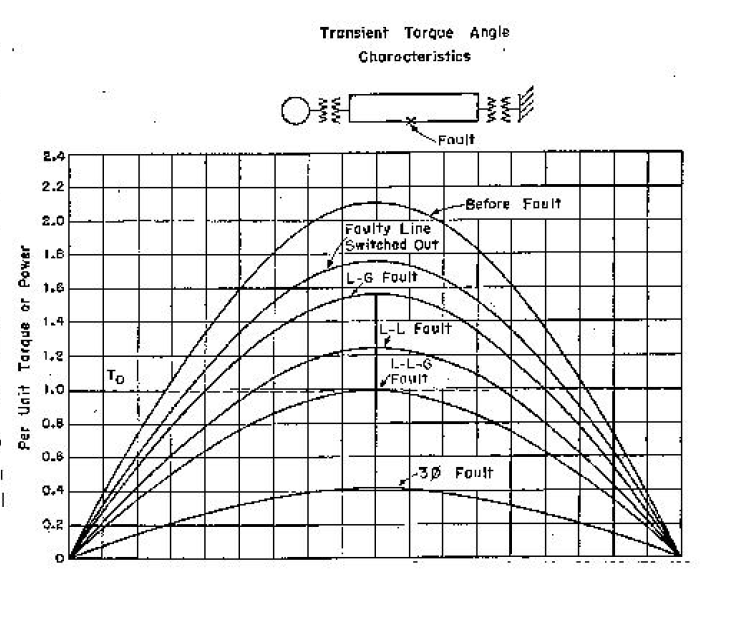
\includegraphics[width=4.0in]{figures/2018s/24q_a.png}}
\caption{Transient Torque Angle}
\label{fig:24q_a}
\end{figure}

\end{enumerate}
\end{document}